\section{Mise en contexte}

Ce document permet d'introduire le protocole 2D-Doc ainsi que la description technique des algorithmes manipulant ce protocole pour le projet. Le protocole 2D-Doc a été créé en 2012 par l'ANTS (Agence Nationale des Titres Sécurisés) à la demande du ministère de l'Intérieur. Pour ce document, il s'agira de la version 04 du protocole qui sera décrite. Ce résumé se concentre uniquement sur la version 04 du protocole.

\section{Le protocole 2D-Doc}

Un code-barres utilisant le protocole 2D-Doc est composé de deux zones principales nommées zone de données et zone de signature. Éventuellement, une zone optionnelle peut être présente et est nommée zone annexe.

\begin{center}
    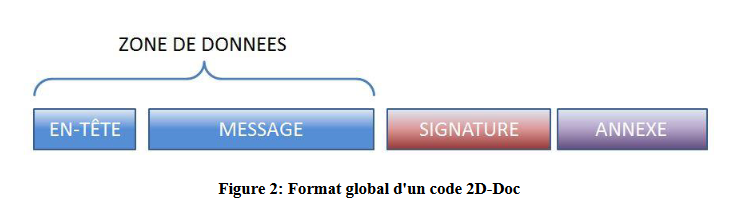
\includegraphics[scale=0.30]{imgs/aa.PNG}\\
    \texttt{Schéma de la structure du protocole 2D-Doc (Source : Documentation 2D-Doc fourni par l'ANTS)}
\end{center}

\subsection{Zone de données}
Dans un premier temps, nous allons nous concentrer sur la zone de données. Cette zone est composée en deux sous-parties, la zone d'en-tête et la zone de message. La zone d'en-tête est de taille fixe et fournit les informations nécessaires pour chaque code 2D-Doc. Cette taille est de 26 caractères alphanumériques au format suivant :

[MI][V][IAC][IC][DED][DCS][CITD][IP][PED]

\textbf{MI (Marqueur d’identification)} : 
Le marqueur doit toujours avoir la valeur DC qui est donc sur 2 caractères.

\textbf{V (Version)} : 
Version de la spécification sur deux caractères numériques, la valeur doit être 04 puisque nous utilisons la version 4.

\textbf{IAC (Identifiant de l'Autorité de Certification)} :
L'identifiant de l'Autorité ayant délivré le certificat sur 4 caractères alphanumériques.

\textbf{IC (Identifiant du certificat)} : 
L'identifiant d'un certificat qui sera utilisé pour signer les données. Il nécessite 4 caractères alphanumériques.

\textbf{DED (Date d’émission du document)} :
Date indiquée par le nombre de jours en hexadécimal depuis le 1er janvier 2000. S’il n’y a pas de date, la valeur est FFFF. Il faut donc 4 caractères alphanumériques.


\textbf{DCS (Date de création de la signature)} : 
Même explication que pour DED.

\textbf{CITD (Code d’identification du type de document)} :
Indique le type du document qui sera encodé en 2 caractères alphanumériques. Exemples : 01 indique un justificatif de domicile, A8 indique un certificat d’immatriculation ou encore B2 pour un résultat de test virologique. 

\textbf{IP (Identifiant du périmètre)} :
La notion de Périmètre permet de ‘répartir dans plusieurs groupes de travail les décisions de définition de type de code 2D-Doc’ et son identifiant sera constitué de 2 caractères alphanumériques. Exemple : 01 pour indiquer un paramètre ANTS.

\textbf{PED (Pays émetteur du document)} :
Représenté sur 2 caractères. Exemples : FR pour France ou IT pour Italie.

Quant à la zone de message, elle est constituée d’une séquence de blocs de données, chaque bloc possédant la structure suivante : \\
\newline
- Un Identifiant de Donnée (ID) sur deux caractères. Cet identifiant permet de connaître la nature de la donnée (sa longueur et son format). \\
- La donnée \\
- D’un éventuel caractère de fin de données <GS> ou de troncature de donnée <RS> \\

La donnée peut être de longueur fixe ou variable selon l'ID, lorsqu’elle est de longueur fixe, on ne peut donc pas faire de troncature. Une donnée de longueur fixe possède la structure suivante : <ID><Valeur du champ>. Lorsqu'elle est de longueur variable, en cas de troncature, le schéma est le suivant : <ID><Valeur du champ après troncature><RS>.
Sinon, le schéma est le suivant <ID><Valeur du champ><GS>.

\textbf{Exemples} :\\
\textbf{2CMARSE<RS>}\\
Avec <RS>, on comprend que la chaine à l’origine de MARSE a été tronquée.\\

\textbf{4114732<GS>}\\
La valeur est ici 14732 et son identifiant est 41.\\

\textbf{2435000}\\
Pas de caractère de contrôle, on comprend donc que c’est une donnée de longueur fixe.\\

\textbf{Note} : Pour chaque type de document pour un périmètre donné, il existe une spécification avec des ID possibles et si la longueur de la valeur associée doit être fixe.

\subsection{Zone de Signature}
La signature présente dans la zone de signature apporte les éléments suivants :

- \textbf{Authentique} : La signature apporte des éléments sur l’identité du signataire \\
- \textbf{Infalsifiable} : La signature ne peut pas être falsifiée \\
- \textbf{Inaltérable} : Les données signées sont inaltérables. Lorsqu’elles sont signées, on ne peut plus les modifier sans corrompre la signature. \\

La signature des données porte sur l’intégralité de la zone de données (en-tête et zone de message). Sa taille est déterminée par l’algorithme utilisé indiqué dans le certificat. La taille minimale de la signature est de 64 octets, pouvant aller jusqu’à 0x7F octets.

En ce qui concerne le format de la signature, elle est ajoutée au format Base32 et est précédée par le caractère <US> pour délimiter la fin de la zone de données et le début de la signature. L’avantage de l’encodage en Base32 est de ne contenir que des caractères affichables qui permet une lecture plus simple pour les APIs de lecture de Datamatrix. En ce qui concerne la génération de la signature, le protocole utilise \textbf{Elliptic curve digital signature algorithm} (ECDSA) qui est un algorithme de signature et plusieurs courbes sont disponibles comme la P-256, P-384 et P-521 qui peuvent être utilisées. La signature se termine obligatoirement par le caractère <GS>.

\subsection{Zone annexe}

Pour cette zone, la structure est la même que la zone de message, son format est identique et permet d’ajouter des données supplémentaires. La différence est que la zone de signature ne prend pas en compte la zone annexe, ainsi, il ne peut être garanti que les informations présentes dans cette zone soient authentiques même en cas de signature valide vérifiée à l’aide d’une API de lecture.

\newpage
\section{Algorithme de lecture | Extraction des données}
Notre outil de scan est capable de lire les datamatrix qui utilisent le protocole 2D-Doc. La structure du protocole ayant été détaillée plus haut, on ne s'attardera pas sur les explications dans cette partie. Nous devons donc dans un premier temps récupérer la partie d'en-tête qui a une longueur totale de 26 caractères. Nous savons en outre quel identifiant fait quelle longueur, l'algorithme va donc lire les 26 caractères en avançant de x caractère (x représentant le nombre de caractère de la valeur associé à l'identifiant), tout en récupérant le contenu et en le vérifiant : 

\begin{center}
    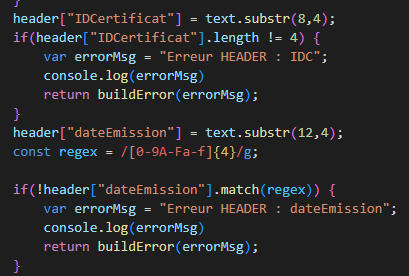
\includegraphics[scale=0.50]{imgs/Capture.PNG}\\
    \texttt{Extrait de l'algorithme vérifiant si le contenu est valide}
\end{center}

Après avoir lu les 26 caractères, on arrive obligatoirement dans le début de la zone de message. Dans cette zone, on récupère les identifiants puis on vérifie si la valeur possède une longueur fixe ou si c'est indéfini. En fonction de cela, on pourra savoir si on doit lire le caractère de troncature/fin de donnée ou s'il n'y a aucun caractère précis à lire car si la longueur est fixe alors il suffit de récupérer la valeur entière sans lire caractère par caractère. L'algorithme est constitué des étapes suivantes : \\
\newline
\textbf{Etape 1 :} \\
- On lit le prochain caractère, si c'est <US>, on passe à l'étape 3 \\
- On lit les 2 prochains caractère en incluant celui-ci qui vient d'être lu et on vérifie si cet ID existe et s'il dispose d'une longueur fixe \\
- S'il existe, on le retire de la liste des ID qui doivent être lu (pour éviter les doublons ou des ID manquants) \\
\textbf{Etape 2 :} \\
- S'il dispose d'une longueur fixe alors on récupère directement la valeur \\
- Sinon, on lit caractère par caractère jusqu'à tomber sur <RS> ou <GS> tout en récupérant le contenu \\
- Retour à l'étape 1 \\
\textbf{Etape 3 :} \\
- On vérifie qu'il existe encore un ID à lire dans la liste des ID car il y a 2 identifiants qui sont interchangeables, ils ne peuvent pas être présent en même temps dans les données (B0 et B1) \\
- Si ce n'est pas le cas, on renvoi une erreur sinon on récupère l'information. \\

L'algorithme prend en compte l'invalidité des données, c'est-à-dire que s'il venait à ne pas trouver <RS> ou <GS> tandis qu'un de ces deux caractères devraient être présent alors l'algorithme renverra une erreur. Il est nécessaire de préciser que notre algorithme ne reconnaît que les identifiants de données pour les justificatifs académiques, si d'autres identifiants sont présent, l'algorithme renverra une erreur. Toutes les données sont sauvegardés dans un tableau.

Après tout cela, on arrivera juste avant la zone de signature. Étant donné qu'elle n'a pas de longueur fixe, nous sommes obligés de récupérer caractère par caractère jusqu'à tomber sur le caractère de fin de signature qui est <GS>. Ensuite, il reste l'annexe mais cette zone n'est pas obligatoire. Dans le contexte de notre projet, il n'a pas été nécessaire de réaliser cette zone mais l'algorithme vérifie quand même si cette zone existe en lisant le prochain caractère, s'il est vide alors il n'y a pas de zone annexe et c'est donc la fin de l'algorithme. Sinon, c'est qu'il existe une zone annexe et dans ce cas, l'algorithme va exécuter les précédentes étapes car la structure étant la même que celle dans la zone de message, l'algorithme reste inchangé pour cette partie.

\begin{center}
    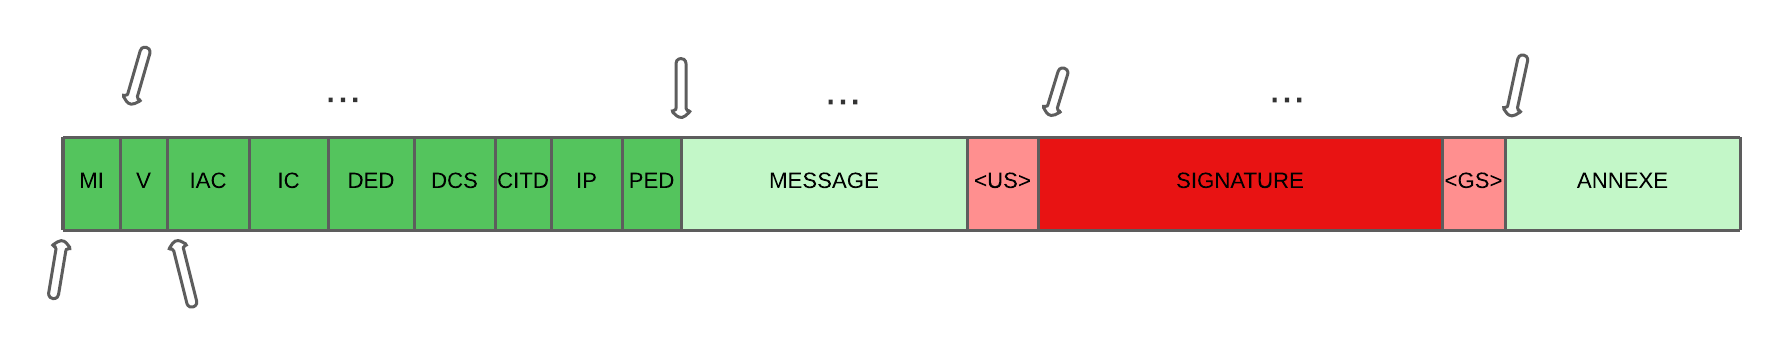
\includegraphics[scale=0.20]{imgs/docTech.png}\\
    \texttt{Schéma détaillé de la structure du protocole 2D-Doc}
\end{center}

\newpage
\section{Algorithme de lecture | Extraction de la signature}

Pour notre projet, nous avons fait en sorte qu'il soit possible de révoquer une signature dans un datamatrix qui utilise le protocole 2D-Doc dans notre outil de création (cf Compte-Rendu ou Notice d'Utilisation). Il a donc fallu réaliser un algorithme qui soit capable de récupérer uniquement la signature. Il y a peu de différence avec l'algorithme de lecture utilisé dans notre outil de scan si ce n'est qu'on ne sauvegarde pas le contenu précédent la signature, on se contente de vérifier si les données sont valides jusqu'à atteindre le caractère <US> qui indique que nous sommes arrivés à la signature. On récupère ensuite le contenu de la signature, c'est-à-dire qu'on va récupérer caractère par caractère jusqu'à tomber sur le caractère <GS> qui indique que nous avons atteint la fin de la signature. De cette manière, seulement la signature est alors extraite du protocole.

\section{Algorithme de Création | Regroupement des données}

Après que nous ayons récupéré toutes les données nécessaires pour générer un datamatrix avec le protocole 2D-Doc, il faut maintenant le construire avec les informations reçues. L'algorithme ici consiste simplement à récupérer l'en-tête, puis le contenu (la zone de message), de créer la signature et de renvoyer le résultat. On récupère l'en-tête et le contenu avec des fonctions qui sont appelés :  
\begin{center}
    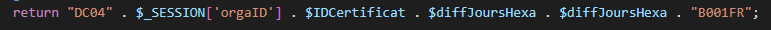
\includegraphics[scale=0.60]{imgs/Capture2.PNG}\\
    \texttt{Valeur de retour pour l'en-tête}
\end{center}

Étant donné que certaines valeurs dans l'en-tête sont définies par défaut, on peut directement les renvoyer en chaîne de caractère (par exemple, DC pour le marqueur d'identification et 04 pour la version du protocole). De cette manière, on récupère les informations nécessaires et nous renvoyons le tout sous forme de chaîne de caractère qui constituera l'en-tête. La chaîne de caractère aura alors une longueur de 26. Il faut ensuite renvoyer le contenu à l'aide d'une autre fonction : 

\begin{center}
    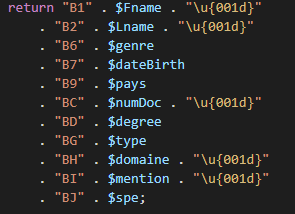
\includegraphics[scale=0.60]{imgs/Capture3.PNG}\\
    \texttt{Valeur de retour pour l'en-tête}
\end{center}

Les ID étant déjà prédéfinis, ils sont donc présents directement dans le code car ces valeurs ne changent pas. On récupère l'ensemble des informations du formulaire en vérifiant que les données sont correctes puis on les concatène aux ID de champ. Selon l'ID, la longueur peut ne pas être fixe, il faut alors préciser le caractère de troncature/fin de chaîne. Pour manipuler les caractères spéciaux en PHP, il faut d'abord préciser qu'il en s'agit d'un avec "$\backslash$u\{\}" puis indiquer quel caractère il s'agit. Ici, 001d correspond à <GS> qui correspond au caractère de fin de données.

\begin{center}
    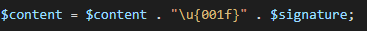
\includegraphics[scale=0.60]{imgs/Capture4.PNG}\\
    \texttt{Valeur contenant l'ensemble des données}
\end{center}

Pour finir, après avoir récupéré l'en-tête et la zone de message, il ne reste plus qu'à les concaténer et générer la signature en utilisant un script Python. Ce scritpt renverra la signature, on aura alors toutes les informations nécessaires pour construire notre datamatrix avec le protocole 2D-Doc. Dans l'image ci-dessus, on concatène "\$content" qui contient l'en-tête et la zone de message au caractère spécial <US> pour indiquer la fin de la zone de message puis on concatène la zone de signature. Comme précisé avant, il n'y a pas de zone d'annexe donc l'algorithme se termine ici.